\documentclass[12pt]{article}
 
\usepackage[margin=.5in]{geometry} 
\usepackage{amsmath,amsthm,amssymb,outlines}
\usepackage{graphicx,tikzsymbols,tcolorbox}
\renewcommand\qedsymbol{$\blacksquare$}
\newcommand{\Sp}{\mathbb{S}}
\tcbuselibrary{most}

\newtcolorbox{newtitle}{
  enhanced,
  colframe=black,
  colback=white,
  boxsep=5pt,
  arc=8pt,
  sharp corners=south,
  borderline={0.5pt}{0pt}{black},
  borderline={1.8pt}{-5pt}{black},
  after skip=30pt
}

\newtcolorbox[auto counter]{statement}[1][]{
  enhanced,
  title={Exercise \ifx\\#1\\\thetcbcounter\else#1\fi},
  colframe=black,
  colback=white,
  colbacktitle=white,
  fonttitle=\bfseries,
  coltitle=black,
  attach boxed title to top left={yshift=-0.25mm-\tcboxedtitleheight/2,yshifttext=2mm-\tcboxedtitleheight/2, xshift=2mm},
  boxed title style={boxrule=0.5mm}
}

\newtcolorbox{newproof}{
  enhanced,
  breakable,
  frame hidden,
  colback=white,
  title={Proof.},
  fonttitle=\bfseries,
  coltitle=black,
  colbacktitle=white,
  boxed title style={boxrule=0.5mm},
  attach boxed title to top left={yshift=-0.25mm-\tcboxedtitleheight/2,yshifttext=2mm-\tcboxedtitleheight/2, xshift=2mm},
  borderline west={1.5pt}{8pt}{black},
  after upper={\hfill $\blacksquare$}
}

\begin{document}

\begin{newtitle}
  \begin{center}
    \textbf{\Huge TDA Homework 1}
  \end{center}
  \textbf{Dahlen Elstran} \hfill \textbf{\today}
\end{newtitle}

\begin{statement}
  Let $f: \Sp^1 \rightarrow \Sp^2$ be a continuous map which is not surjective. Prove that it is homotopic to a constant map.
\end{statement}
\begin{newproof}
  If $f$ is not surjective, then there exists some $x \in \Sp^2$ such that $x \notin f(\Sp^1)$. So we can consider 
  $f(\Sp^1)$ to be $\Sp^2 \setminus \{x\}$, which is homotopy equivalent to a point:
  \par \begin{center} 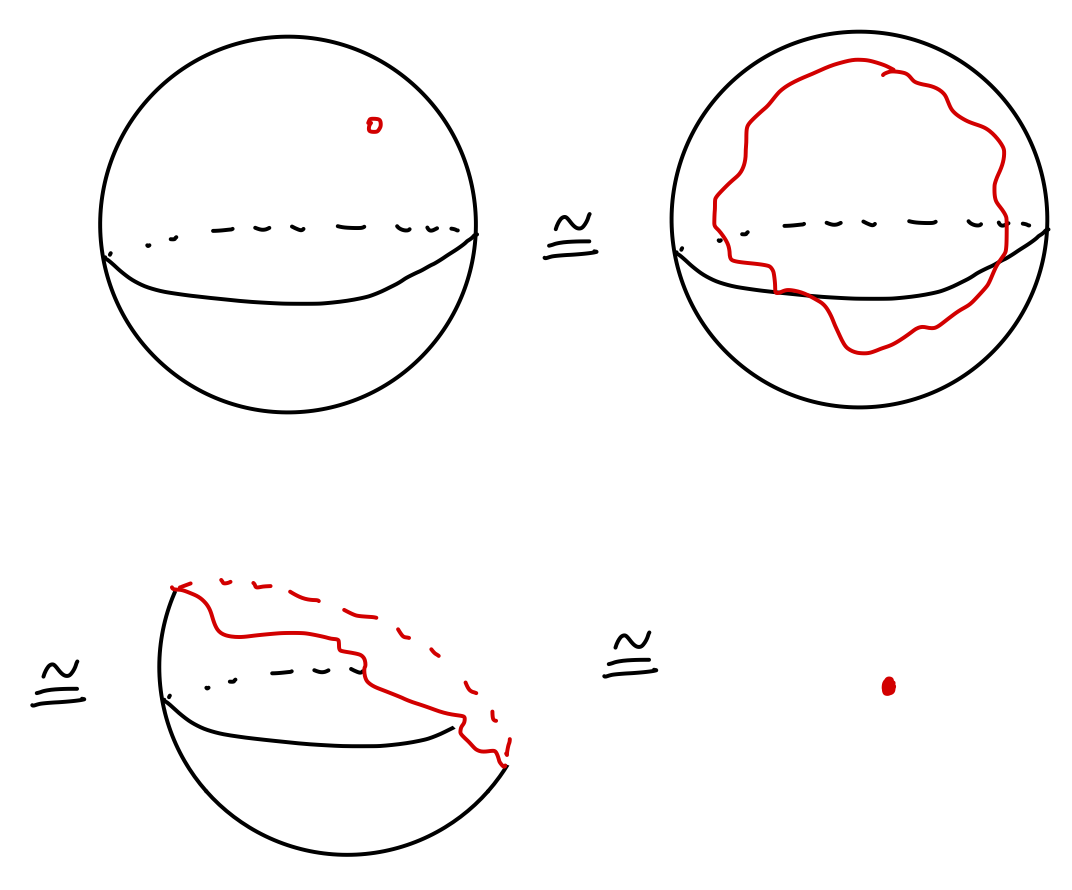
\includegraphics[scale=.2]{1-1.png} \end{center}
  Thus every map in $f(\Sp^1)$ is homotopic to a constant map. 
\end{newproof}

\begin{statement}
  Let $X$ and $Y$ be two homeomorphic topological spaces. Show that if $X$ has dimension $n$, then $Y$ also has dimension $n$.
\end{statement}
\begin{newproof}
   Consider a homeomorphism $f: Y \to X$, and then let $y \in Y$ with $x = f(y)$. Because $x \in X$, $x$ must have dimension 
   $n$, so that there eists an open set of $X$, call it $O$, containing $x$ with a homeomorphism $h: O \to \mathbb{R}^n$. 
   Then, we can let $O'=f^{-1}(O)$, and note that it is an open set of $Y$ containing $y$. We also know that 
   $h \circ g: O' \to \mathbb{R}^n$ is a homeomorphism, and so $Y$ has dimension $n$.
\end{newproof}

\begin{statement}
Let $(G,+)$ be a group. Prove that
    $$ \forall g \in G, g+g = 0 \Rightarrow G \hspace{0.2cm} \text{is commutative}.$$
\end{statement}
\begin{newproof}
  Let $g_1,g_2 \in G$, and note that $g+g=0 \iff g=-g$. Then 
  \begin{align*}
    (g_1 + g_2) + (g_1 + g_2) &=  0 \\
    g_1 + g_2 & = -(g_1 + g_2) \\
    g_1 + g_2 &= (-g_2) + (-g_1) \\
    g_1 + g_2 &= g_2 + g_1
  \end{align*}
  Thus the group is commutative.
\end{newproof}

\begin{statement}
   Characterize the two surfaces depicted in Figure 1  in terms of genus, boundary, and orientability.
   \par \begin{center} 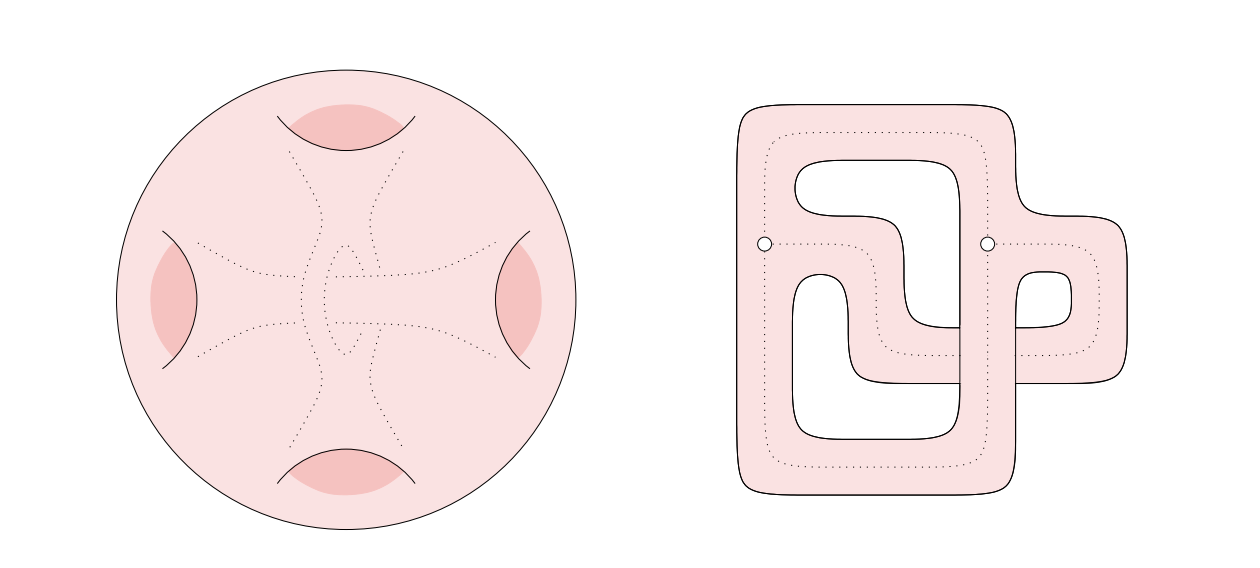
\includegraphics[scale=.5]{4-1.png} \end{center}
\end{statement}
\begin{newproof}
  For the first surface, it clearly has no boundary and is non orientable. It's genus is 3, which can be found by using 
  the Euler characteristic, or by seeing the 3 handles, which in the figure presented, are the tunnels in the middle.
  \par For the second surface, it has boundary because, as this diagram shows,
  \par \begin{center} 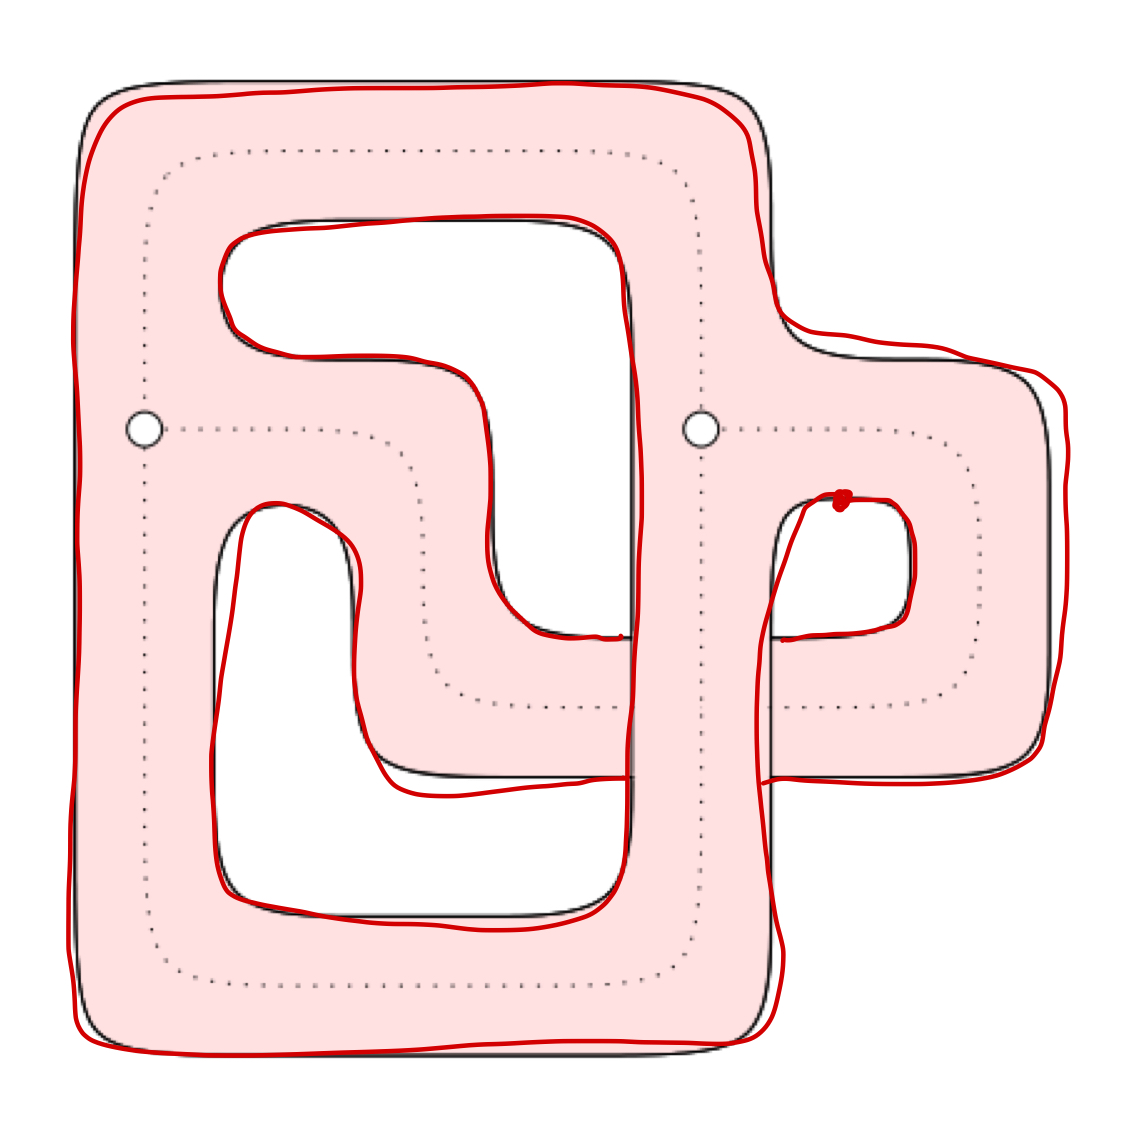
\includegraphics[scale=.1]{4-2.jpg} \end{center}
  you can see there is only one continuous line on the entire boundary. The surface is orientable as well, as there is a 
  distinct top and bottom. As for the genus, we can use the equation $\chi=2-n-b$, where $\chi$ is the Euler characteristic,
  $n$ is the genus, and $b$ is the boundary. We know $\chi$ to be $V-E+F=2-3+0=-1$ and $b$ to be $1$, so the genus must be $2$.
\end{newproof}

\begin{statement}
  Is every graph that can be embedded on the Mobius strip planar?
\end{statement}
\begin{newproof}
  No. A counterexample would be $K_{3,3}$, which is not planar: 
  \par \begin{center} 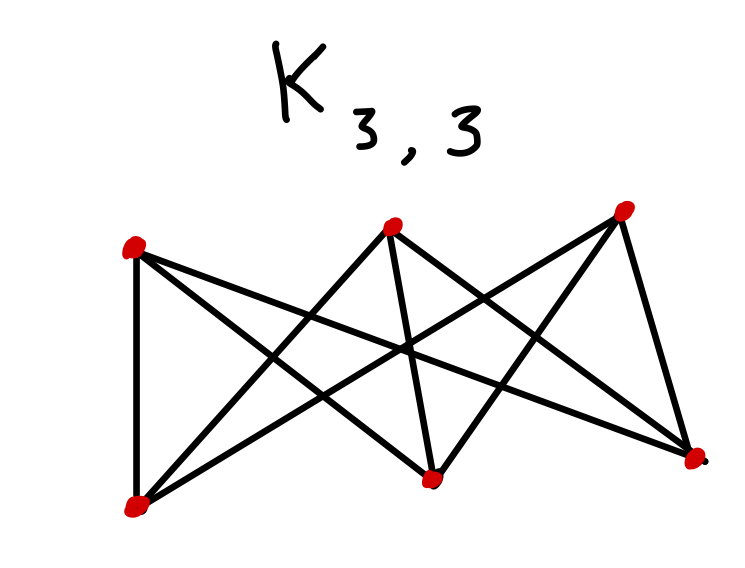
\includegraphics[scale=.2]{5-1.png} \end{center}
  However, it can be embedded on the Mobius strip.
\end{newproof}

\end{document}
